\section{Discussion}

\begin{comment}
\textcolor{blue}{I think this belongs better to Discussion section, not here.
There are three types of programmers in the world: 
1) Those who are comfortable participating on a site in English. They won't be affected by the existence of SO in other languages. 
2) Those who can read English but not express themselves. Most developers can understand some English as the most programming languages are written in English. But being able to understand what a few select words (i.e., as a programmer) does not necessarily mean being proficient enough in a language to read or write. Therefore, some developers even though can read and write English without any problems prefer to ask or answer questions in their native language. Let's bring Yukihiro Matsumoto\footnote{\url{https://en.wikipedia.org/wiki/Yukihiro_Matsumoto}} (also known as Matz, he's the inventor of Ruby, one of the most popular programming languages in the world) and Ruby as an example. Matz knows English and has given several talks in English but yet he still got his programming blog in Japanese. And at the beginning of Ruby, most of its documents are also in Japanese. They can benefit from Stack Overflow, but they can't contribute. 
3) Those who can't speak English at all. They can't even benefit from Stack Overflow.
According to our empirical study in this section, creating SO sites in other languages does attract programmers of type 2. 
But they weren't contributing much to Stack Overflow in the first place, so Stack Overflow isn't losing too much by it.
}
\end{comment}

Our study not only provides the evidences to validate the users' concerns about multi-lingual Q\&A sites, but also reveals some needs for better supporting multi-lingual Q\&A sites.
Fig.~\ref{fig:linkExample} shows an example in which a user asked a question in RSO but received no answer timely.
And then, the user managed to find a duplicate question in English Stack Overflow (Fig.~\ref{fig:ESOanswerExample}) which can perfectly answer his question in Russian Stack Overflow.
This user went back to Russian Stack Overflow and answered his own question (Fig.~\ref{fig:RSOanswerExample}) in which he referenced to the ESO question and translated the accepted answer of that ESO question in his post.
Such cases further demonstrate the needs of cross-site retrieval and translation which are discussed in this section.

%In this section, we discuss two such needs: cross-site retrieval and cross-site translation.

\begin{figure}
	\centering
	\subfigure[\#638741: A RSO post that references to and translates a duplicate ESO question]{  
		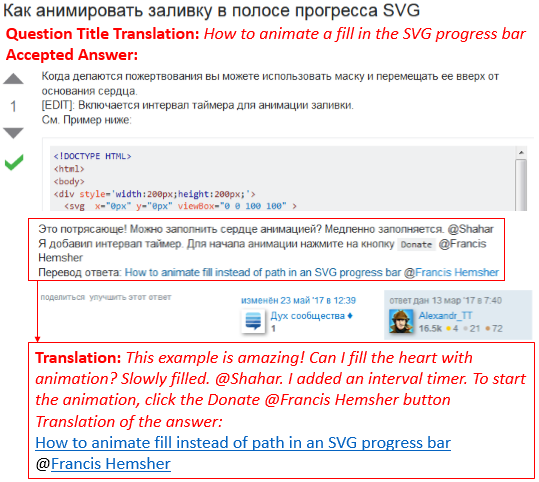
\includegraphics[width = 0.48\textwidth]{figures/exmp1.png}
		\label{fig:RSOanswerExample}}
	\hfill
	\subfigure[\#42672537: The referenced ESO question with the accepted answer]{  
		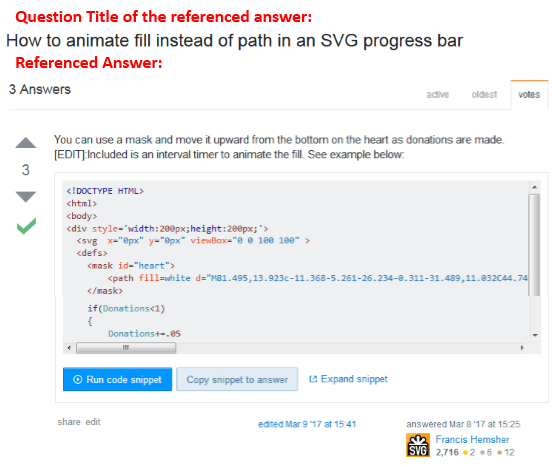
\includegraphics[width = 0.48\textwidth]{figures/exmp2.png}
		\label{fig:ESOanswerExample}
	}
	\caption{An example of manual cross-site linking and translation}
	\label{fig:linkExample}
\end{figure}

\subsection{Cross-site Retrieval}
\label{sec:crossLinking}
Since its launch in 2007, English Stack Overflow has accumulated a large pool of computer programming knowledge, including 16 million questions and 24 million answers.
In contrast, the non-English Stack Overflow sites have been launched in recent years.
As the non-English Stack Overflow users and the English Stack Overflow users do share some common interests, it is very likely that some questions asked on a new non-English Stack Overflow site may have been already asked or even answered on the English Stack Overflow.
If we can recommend relevant, high-quality questions and answers (e.g., accepted or highly-voted by the community) on English Stack Overflow to the users of the new non-English Stack Overflow site, it will benefit the new site.

There are two types of users in a multi-lingual Stack Overflow site: those speak only the native language, and those can at least read some English.
For the users who can read some English, the recommendation will lead them to the relevant posts on English Stack Overflow which directly satisfy their information needs.
For the users who speak only the native language, even though they cannot understand the English descriptions, they can at least understand some code snippets or APIs mentioned in the English posts, which are the real ``meat'' of computer programming knowledge.
Therefore, these non-English speaking users can still benefit from the recommendation of relevant English posts.

However, it is not an easy task to retrieve duplicate or related posts across multi-lingual Stack Overflow sites for two reasons.
First, there is a natural language gap between non-English Stack Overflow and English Stack Overflow.
%, considering most users' English in the non-English Stack Overflow.
Second, there are too many posts in Stack Overflow to retrieve related posts, and these post themselves often have lexical gap, i.e., they discuss the same computer programming knowledge but use very different words~\cite{chen2016learning}.
So an effective cross-site retrieval tool is needed.

Our cross-site retrieval method in the last section has the potential to be adopted for this purpose, as it can bridge both the language gap and lexical gap to certain extent.
To validate this potential, we use the 50 Russian \textit{Python} questions that have manual hyperlinks to ESO posts in Section~\ref{sec:explicitLink} as query questions to retrieve relevant ESO questions from the question database of 779,370 English \textit{Python} questions.
For 29 (58\%) of these 50 Russian \textit{Python} questions, the retrieved top-10 ESO questions by our method contain the ESO posts that RSO users manually hyperlink in the 50 Russian \textit{Python} questions.
%The results show that 29 (58\%) of the ground truth are in the top-10 recommendations.
For the rest 21 Russian questions, we further analyze the human-hyperlinked ESO posts that our method fails to retrieve in the top-10 ESO questions.
For example, the RSO question ``\foreignlanguage{russian}{Порядок удаления элементов списка в python}''\footnote{\url{https://ru.stackoverflow.com/questions/55464/}} (``the removal of elements of the list in python'') has a hyperlink to an ESO question ``Calling del on a list''\footnote{\url{https://stackoverflow.com/questions/8205102/}}.
In this example, ``del'' is a function name for deleting.
However, our method currently cannot reliably capture such domain-specific information and sentence-level semantics.

Therefore, although promising, our cross-site retrieval method still need to be enhanced, for example, replacing the current word-level semantic modelling with more advanced sentence-level semantic methods~\cite{kiros2015skip, conneau2017supervised} for better performance. 
Furthermore, our current analysis is anecdotal.
More formal evaluation should also be carried out to validate the effectiveness and efficiency of a cross-site retrieval method.

\subsection{Cross-site Translation}
\label{sec:crossTranslation}
Although cross-site retrieval across multi-lingual Q\&A sites is useful for users, it is just the first step, not the ultimate solution.
To assist non-English speaking users in fully exploiting the existing knowledge in English Stack Overflow, some English questions and answers especially those highly-viewed, highly-voted ones should be translated into other languages.
It was also mentioned in some comments on the announcement of multi-lingual Stack Overflow sites, such as ``\textit{I think a better idea would be to let the community translate each question and answer--think of it as a kind of editing capability.}'', ``\textit{...If someone finds a really good question on a site, with a good answer, they can translate it to other sites, post it on those sites (cite the original of course)...}''.

Breaking the language barrier would make the entire world more knowledgeable, and even users who cannot speak English at all can fully benefit from the knowledge on English Stack Overflow.
As translating could cost less effort than drafting an answer as good as the well-examined one on English Stack Overflow, it may save much effort of core users in the multi-lingual site who serve as the backbone for the relatively new site.

Recently, machine translation has made big progress by incorporating deep learning methods~\cite{wu2016google, sutskever2014sequence}. 
To assist high-quality translation, we can adopt the power of advanced machine translation to first obtain an overall translation, and then let human users revise the translation.
However, the general machine translation system may not work well for Q\&A discussions, and it needs to be improved in two aspects.
First, current machine translation models focus on sentence-level translation without contextual information.
However, to translate an answer well in a Q\&A discussion thread, the model not only needs to consider the current sentence in the answer, but also needs to take the corresponding question information into consideration.
Second, Stack Overflow is a domain-specific site about computer programming, while the current machine translation system is trained for general purpose.
Many domain-specific words will be out of vocabulary or have different meanings from daily life such as ``bug'', ``port'', etc.
So the general machine translation model must be customised by incorporating the domain-specific knowledge.

In addition to technical aspect of cross-site translation, we also need to design some mechanisms to motivate users to contribute to the translation activity.
We can set up a reward rule that once users translate one answer from English Stack Overflow to non-English site, they can earn some award points.
Once other users vote their translated answer, they will earn more points and reputation score.
A translator badge can also be created and awarded to users whose translation score reaches to a certain level.

\begin{comment}
\subsection{Guideline to other Q\&A sites}
\textcolor{red}{CCY: Maybe we talk about how our discovery in Stack Overflow can help guide the development of multilingual variants to other similar Q\&A sites. Or we may talk about the similar situation of Quora.}

\textcolor{blue}{I think this belongs to here.
	There are three types of programmers in the world: 
	1) Those who are comfortable participating on a site in English. They won't be affected by the existence of SO in other languages. 
	2) Those who can read English but not express themselves. Most developers can understand some English as the most programming languages are written in English. But being able to understand what a few select words (i.e., as a programmer) does not necessarily mean being proficient enough in a language to read or write. Therefore, some developers even though can read and write English without any problems prefer to ask or answer questions in their native language. Let's bring Yukihiro Matsumoto\footnote{\url{https://en.wikipedia.org/wiki/Yukihiro_Matsumoto}} (also known as Matz, he's the inventor of Ruby, one of the most popular programming languages in the world) and Ruby as an example. Matz knows English and has given several talks in English but yet he still got his programming blog in Japanese. And at the beginning of Ruby, most of its documents are also in Japanese. They can benefit from Stack Overflow, but they can't contribute. 
	3) Those who can't speak English at all. They can't even benefit from Stack Overflow.
	According to our empirical study in this section, creating SO sites in other languages does attract programmers of type 2. 
	But they weren't contributing much to Stack Overflow in the first place, so Stack Overflow isn't losing too much by it.
}
\end{comment}

\begin{comment}
\textcolor{red}{Some quotes from users' comments.}
I think a better idea would be to let the community translate each question and answer--think of it as a kind of editing capability. 
You don't need a formal system in place to do that. If someone finds a really good question on a site, with a good answer, they can translate it to other sites, post it on those sites (cite the original of course) and then, if other users find it valuable, they can then vote on the translated version. If the content is not useful, they don't get rep, if it is, they do, based on votes. This would encourage the translation of the quality content, and discourage the translation of the crap.
But a GREAT IMPROVEMENT would be creating an auto-translate system to all Stack Exchange websites, which means: any text that is not inside a `code` block would be viewed in the user's language. It'd be great mainly because currently a lot of good questions/answers are only known to a particular language, so breaking the language barrier would make the entire world more knowledgeable. The option to view it in the original language or use other translation engines (provided externally, fecthing through Javascript) would be a plus. Anyway, congratulations in joining Portuguese and Japanese in the seemly growing Stack Overflow languages websites group :)
Maybe a good idea would be to award points to users willing to translate answers from the english version into portuguese; a translator badge could be created even. My one bit of criticism is that my reputation from stackoverflow didn't move over to the portuguese version. I kinda expected that.
This is the world wide web and it is built on a thing called hypertext. Multiple languages? Cool, that's the "world" part. But don't forget about hypertext. Please, make sure that questions and answers can be linked easily across the different language sites. If someone asks a question in Japanese that is essentially a duplicate of an existing English question, linking the two questions will allow Japanese speakers (who might understand *some* English, or at least be able to read code snippets) to get immediate value from past answers, without waiting for new answers and without waiting for translation. Although such links would also aid translators.
This could be the first step towards a multilingual stack exchange. Where every site is available in every language. There shouldn't be a language version of stackoverflow, instead stackoverflow should have built in support for different languages and a workflow for translating into all of those languages. With the help of translation, both machine and human, the knowledge that non English speakers have can be shared with English speakers and vice versa.	
\end{comment}
